\documentclass{article}
\usepackage[utf8]{inputenc}
\usepackage{graphicx}

\title{Memory}
\author{MCB C61 with Professor David Presti \\ \\ Benjamin Lee}
% \date{8 March 2018}

\begin{document}

\maketitle

\textbf{Key Concepts:}
\begin{itemize}
    \item pi
    \item \textit{The Mind of a Mnemonist}
    \item Synesthesia
    \item Memory: working or short-term, long-term
    \item Consolidation
    \item Amnesia: retrograde, anterograde
    \item Dementia: Vascular, Alzheimer's
    \item Drugs and meomry impairment
    \item Nootropic drugs
    \item Karly Lashley
    \item Donald Hebb
    \item Patient H.M.
    \item Hippocampus
    \item Memory: declarative, non-declarative
    \item \textit{Aplysia Californica}
    \item Eric Kandel
    \item Gill-withdrawal learning
\end{itemize}

\newpage
\section{Pi $\pi$}
The ratio, for any circle, of the circumference to the diameter 
\begin{itemize}
    \item Shows up in many mathematics and physics places: Maxwell's equations in electromagnetism, Einstein's gravitational field equations in general relativity, the Schrodinger equation and Heisenberg uncertainly relations in quantum mechanics, descriptions o f vibrating or periodic motion of all sorts. 
    \item Pi is an irrational number: cannot be represented as a ratio of two integers 
    \item Value of Pi can never be computed exactly
    \item Approx. $\pi$ as 3.14, ten decimal places 3.1415926535
    \item Calculated Pi to ten trillion ($10^{13}$) decimal places
\end{itemize}

\noindent\textbf{Human memory and Pi $\pi$} \\
World record for memorizing digits of $\pi$
\begin{itemize}
    \item In 1973, 930 digits, then 1,111, then 1210
    \item By 1978, 10,000 digits
    \item by 1980, 20,013 digits
    \item From 1987 to 2005, world record held by two individuals from Japan: first 40,000 digits and then 42,195
    \item In 2005, Lu Chao, 24 yr old student from China, 67,890 digits. Planned to recite 90,000 after memorizing 100,000
        \subitem Recited for over 24 hours. Sleep deprivation and fatigue made him make a mistake 
\end{itemize}

\newpage
\section{\textit{The Mind of a Mnemonist}}
1965 book by Russian neuropsychologist Alexander Luria (1902 - 1977) \\

Luria describes his investigations of a man he met in the 1920s and knew for more than thirty years. Solomon Shereshevsky (1886 - 1958) called "S" in the book, worked as a newspaper reporter when he first came ot Luria's attention. S could recall exact details of events, including conversations, years after they happened. Luria found that S could recall very long lists of numbers, letters, or words, without error, years after being asked to learn them. 

\begin{itemize}
    \item S had profound \textbf{synesthesia}, characterized by unusual blending of perceptions between different sensory modalities
    \item Sounds may evoke experiences of colors
    \item letters, words and numbers may evoke experiences of color, sound, taste, smell, and texture
\end{itemize}

"Usually I experience the word's taste and weight, and I don't have to make an effort to remember it - the word seems to recall itself. But it's difficult to describe. What I sense is something oily slipping through my fingers .. or I'm aware of a slight tickling in my left hand caused by a mass of tiny, lightweight points. when that happens I simply remember, without having to make the attempt." \\ 
(no effort in memorizing because it comes clear like a picture in front of them or some key evocation that connects the experience with the memory profoundly) \\

\newpage
\section{Memory: Short term vs Long term}
Memory can be deconstructed into two major components: working memory (aka short-term memory) and long-term memory. \\ 

\subsection{Shot-term Memory (STM) aka Working Memory (WM)}
\begin{itemize}
    \item Tends to last from seconds to a few minutes (can last indefinitely if you keep thinking) 
    \item Limited capacity: can only hold so many items in STM. (generally fewer than 10) 
    \item Can measure by having people repeat back a list of numbers or words immediately after hearing them
\end{itemize}

\subsection{Long-term Memory (LTM)}
Memories that have been retained in some more permanent manner are stored in LTM
\begin{itemize}
    \item Variety of pathways to get information into LTM
    \item Rehearsing items in WM or short-term (process by which people would memorize the digits of $\pi$
    \item Repetition assists in encoding memories into LTM
    \item Easier to remember people we see more often, streets and numbers we refer to, lectures and books we review for class
    \item Some information is easily stored in LTM, for example, when they have significant meaning or emotional salience
    \item "understanding", forming links between information already known
\end{itemize}

\noindent Long-term Memory involves information storage and retrieval. new memories are frail, while things that happened years ago are easier to remember\\

\noindent \textbf{Consolidation:} the process where new memories become more stable and robust with time. 

\begin{itemize}
    \item Retrieval involves some mechanism of access to the stored memory 
    \item Forgetting is because of failure of either storage or retrieval 
    \item Info can be registered in WM, but never retained in LTM
    \item LTM can decay or be lost over time
\end{itemize}

\subsection{Amnesias}
Pathological memory problems are known as amensias and there are two major categories: retrograde and anterograde amnesias. 

\begin{itemize}
    \item \textbf{Retrograde amnesia:} an inability to recall events \textit{before} the onset of the amnesia
        \subitem Memories of past experiences are lost or unable to be retrieved from LTM
    \item \textbf{Anterograde amnesia:} an inability to recall events \textit{after} the onset of the amnesia, such experiences are not retained in LTM  
        \subitem Really a problem with learning new information rather than remmbering what is already there
\end{itemize}

\noindent Amnesia may be associated with various physical injuries to the brain 
\begin{itemize}
    \item Cellular damage from stroke or seizure
    \item Brain tumor
    \item Infection (encephalitis) 
    \item Traumatic injury sustained in an accident
    \item Surgical excision of brain tissue
    \item Electroconvulsive shock therapy (ECT): a psychiatric procedure in which seizures are induced in a  patient, with the goal of reducing symptoms of depressed mood (produce retrograde amnesia)
\end{itemize}

\subsection{Dementia}
\textbf{Definition:} a neurological condition characterized by global loss of cognitive abilities - not only memory but other capacities, such as attention, judgment, planning, problem solving, and motor coordination. 

Generally begins with anterograde effects, inability to remember new info, then if it is sufficiently severe, retrograde memory loss may eventually develop. Severe dementia is a deteriorating condition and can result in loss of sense of self. \\

\noindent \textbf{Two common forms:}
\begin{itemize}
    \item \textbf{Vascular dementia:} associated with the accumulation of cellular damage in the brain related impaired blood circulation
        \subitem Generally due to atherosclerosis or repeated small strokes
    \item \textbf{Alzheimer's dementia:} associated with the presence in the brain of what are called senile plaques (extracellualr deposits of aggregates of polypeptide called beta amyloid) and tangles (aggregates of tau protein, a protein involved in the assembly and stabilization of microtubules) 
        \subitem Ultimate causes of this condition and how to prevent its onset are not presently understood 
\end{itemize}

\section{Drugs and Memory Impairment}
Many drugs are related to memory impairment during use
\begin{itemize}
    \item Sedative-hypotics: alcohol, benzodiazepines, and others can produce temporary anterograde amnesia
    \item "alcoholic blackout": a state of intoxication where the drinker is engaging and awake but has no memory of the events  the next day
    \begin{itemize}
        \item Information never stored in LTM
        \item Heavy alcohol consumption over extended periods of time also associated with permanent memory impairment
    \end{itemize}
    
    \item The benzodiazepine, Midazolam (Versed), is sometimes given in conjunction with medical procedures in which the patient is only partially anesthetized
    \begin{itemize}
        \item Anterograde amnesic properties of midazolam i pair the person's ability to remember any potentially uncomfortable parts of the procedure
        \item Treats anxiety, helps with sleep, gets complaints of memory impairment
    \end{itemize}
    \item Nonbenzodiazepine hypnotics prescribed for insomnia, Zolpidem (Ambien), zaleplon (Sonata), and eszopiclone (Lunesta), can produce antergrade amnesia
    \begin{itemize}
        \item Reports of people engaging in strange or dangerous behaviors
        \item Cooking and eating in the middle of the night
        \item Driving a car in their pajamas
        \item Not roused at all, state of consciousness or unconsciousness?
    \end{itemize}
    
    \item Other memory impairment drugs include cannabis (marijuana), cholesterol-lowering drugs (statins), antiseizure medications, opiods, beta-blockers (hypertension), older-generation antihistamines (Benadryl), anticholinergics (treats urinary incontinence (lack of control)), and tricyclic antidepressant medications. 
    \subitem Used to treat elderly individuals, which may result in mental confusion in elderly
\end{itemize}

\noindent \textbf{Nootropic:} term used to describe drugs claimed to improve aspects of cognition, including memory. 
\begin{itemize}
    \item Claims have been made for caffeine, nicotine, arecoline, and amphetamine
    \item Chemicals that influence acetylcholine neurochemistry have received particular attention
    \item Phosphatidylcholine (lecithin), the phospholipid precursor to the synthesis of acetylcholine; and various inhibitors of acetylcholinesterase, enzyme for breaking down acetylcholine. 
    \item Drugs that reduce memory loss associated with Alzheimer's and other dementias: donepezil (Aricept), tacrine (cognex), rivastigmine (Exelon), and galatamine (Razadyne) and red spider lily (\textit{Lycoris radiata})
\end{itemize}

\newpage
\section{Important Figures}

\subsection{Karl Lashley (1890 - 1958)}
Addressed the question: are memories stored in some particular part of the brain? \\ 
Studied the ability of rats to navigate in mazes - how to go from start to finish without making wrong turns and entering blind alleys - for which they were rewarded with treats \\ 

Lashley then made lesions to various places in the rat's cerebral cortex and measured their effects on performance in the maze. He found that lesioned rats made errors in navigating the maze, as if their memory for the maze had been damaged. Number of errors made in navigating the maze was proportional to the size of the cortical lesion, but not its location in the cortex. \\

Lashley concluded that \textbf{memory} was not localized ito any \textbf{particular region} of the cerebrum. 

\subsection{Donald Hebb (1904 - 1985)}
Suggested that networks of many neurons, extending throughout the cerebral cortex, represent the information stored in memory. \\

\textbf{Memory} is \textbf{distributed}; somehow large portions of the brain work together in the formation of and retrieval of memories. For example: memories contain multiple kinds of sensory and emotional information, such as a favorite restaurant, which can be composed of several tastes, smells, sights, actions, etc. 

\subsubsection{Patient H.M. aka Henry Molaison (1926-2008)}
Patient studied for over 50 years by psychologist and neurologists and for reasons of privacy was always referred to by initials in dozens of scientific publications. When he died in 2008 at age 82, his identity was revealed to the world \\

Henry had seizures beginning at age 10. Epilepsy was idiopathic (unknown). May have been related to hitting his head in a bicycle accident. Maybe Genetic risk. \\
Henry's seizures became increasingly frequent and severe. Candidate for brain surgery in his 20's. \\

1953, underwent surgical removal of portions o f his medial temporal lobs, including \textbf{hippocampus}, and adjacent entorhinal cortex and amgdala from both hemispheres of his brain. \\ 
His epilepsy decreased, but had profound impairment of memory. (reported in 1957 by William Scoville, surgeon who performed surgery, and Brenda Milner, neuropsychologist who studied with Hebb and Penfield. \\ 

He had normal working memory and could remember stuff from before his surgery, but he was unable to remember for more than a few minutes, any new information acquired after his surgery. Suffered from profound anterograde amnesia. \\ 
Could have had a conversation with his doctors but had no recollection of that conversation the next time they met. \\ 

\noindent \textbf{Hippocampus:} highly \textbf{interconnected} with all other regions of the cerebral cortex with interconnectivity running in both directions (both sides of cortex). This \textbf{communication} appears to be central to \textbf{organizing, storing and consolidating memory}, with the hippocampus serving as a hub of distributed activation that somehow helps to form the networks of cortical neural connections involved in representing memories in the brain. (also reason why this place is frequent focus of seizures) 

H.M. could still learn and remember; for example, an experiment where H.M. drew a path of the same maze everyday and got better, but never recalled ever seeing the maze. 

\newpage
\section{Declarative and Nondeclarative Human Memory}
\begin{itemize}
    \item \textbf{Declarative memory:} can be brought to mind in words or describable images. 
        \subitem includes facts and other informational type knowledge (semantic memory), as well as specific time-and-place events from one's experience (episodic memory) 
    \item \textbf{Nondeclarative memory:} includes procedural memory, classical conditioning and priming. 
        \subitem H.M. could accomplish this kind of learning and remember what he learned, with no awareness of it. 
\end{itemize}

\begin{figure}[htp]
\centering
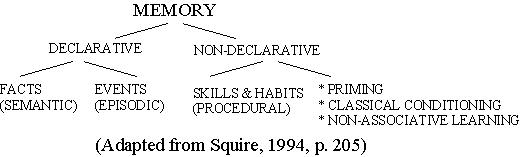
\includegraphics[width=\textwidth]{images/tulving_model.jpg}
\caption{Tulving Model of Memory}
\label{fig: Tulving}
\end{figure}

\begin{itemize}
    \item \textbf{Procedural memory} involves performing a sequence of actions, such as maze tracing, riding a bike, typing, swimming, etc
    \item Can't describe well, "just do it" kind of task
    \item \textbf{Classical condition} is learning to associate together certain stimuli and responses
    \item Beep sounded before puff of air, we associate puff with the beep and will instinctively blink at the sound of beep if we are conditioned with the air puff. 
    \item \textbf{Priming:} when exposure to stimulus influences one's response to future exposures to this stimulus. (central to advertising)  
\end{itemize}

\newpage
\section{Hebbian Learning}
"When an axon of cell A is near enough to excite a cell B and repeatedly or persistently takes part in firing it, some growth process or metabolic change takes place in one or both cells such that A's efficiency, as one of the cells firing B, is increased" \\ 

Repeated activation of a network strengthens the synaptic connections within the network. Neuroplasticity!\\
\begin{center} 
\textbf{"Neurons that wire together, fire together" -Cog Sci 1}
\end{center}

\subsection{Eric Kandel and \textit{Aplysia Californica}}
Conducted an experiment detailing Hebb's idea with the \textit{Aplysia Californica} or sea hare. Study describes the molecular mechanism related to the short-term and long-term strengthening of synapses regulating the reflexive behavior of gill withdrawal. \\ 

\noindent \textbf{Gill Withdrawal Learning:} 
\begin{itemize}
    \item Respiratory gill on \textit{Aplysia} attached to structure called siphon
    \item If siphon is touched, sensory neurons send signals that rapidly retract the gill into the mantle cavity, protecting the gill from injury
    \item 
    \item Electric shock applied to tail at the same time as touching the siphon, an increased robustness of gill withdrawal in response to touch observed. 
    \item increases relation link of siphon sensory neurons with motor neurons mediating retraction of gill. 
\end{itemize}

\noindent \textbf{Chemical Process of Gill Retraction} \\
Serotonin activates G-protein-coupled serotonin receptors, initiating the following sequence of events
\begin{itemize}
    \item activated G-protein
    \item activated adenylate cyclase 
    \item increased cAMP synthesis
    \item activated cAMP dependent protein kinase A (PKA) 
    \item phosphorylated potassium-leak channels located in the membrane of the axon terminal 
    \item closed potassium-leak channels 
    \item decreased outward K$^+$ current
    \item prolonged depolarizing phase of action potential
    \item voltage-gated Ca$^{++}$ channels opened longer 
    \item greater Ca$^{++}$ influx into axon terminal 
    \item increased release of glutamate neurotransmitter 
    \item increased exitation of postsynaptic motor neuron mediating gill retraction
\end{itemize}

\begin{figure}[htp]
\centering
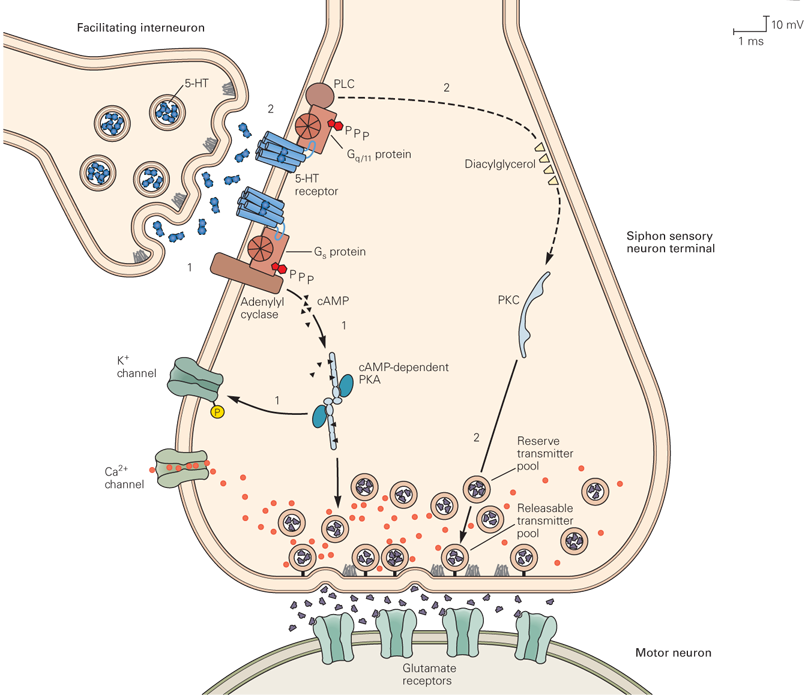
\includegraphics[width=\textwidth]{images/seaharesynapse.png}
\caption{Synaptic connections in \textit{Aplysia californica}}
\label{fig: Sea Slug}
\end{figure}

Repeated activation of serotonin receptors results in high intracellular levels of cAMP, leading to more sustained activation of PKA. PKA remains activated longer even in the absenc of cAMP. Produces persistent elevation of glutamate neurotransmitter release onto the motor neuron controlling gill withdrawal. (read book for more indepth explanation)
\newpage
Lecture Notes:

Working Memory (WM) (Short Term Memory) (STM)
limited capacity transient

Long Term Memory (LTM)
initially fragile
consolidation (neural plasticity??) (from STM to LTM) (Hippocampus to long term storage somewhere) (sleep is key to consolidation) 
structural change (not localized, distributed)

Karl Lashley (1890 - 19558) 
rat maze in 1920's
cut up the rats brain


H.M. Henry Molaison (1926-2008)
severe seizures since age 10, surgery at age 27, 1953
Removed his hippocampus because his seizures were thought to be amplified by the hippocampus, which distributes info throughout the brain

WM ~okay
old LTM ~okay
could not learn new information
hippocampus as hub of distributed storage and consolidation

declarative  

nondeclarative
ex: riding a bicycle

Structural change inn neural networks 
Danald Hebb (1902-1985) 
Hebbian learning (neuroplasticity) 
Aplysia californica (sea slug, sea hare) 
shock siphon or gill of sea slug
Following a single aversive stimulus to tail, synaptic strengthening lasts ~ one hour (STM) 
Found K$^+$ leak channels 




\end{document}